Software languages, crucial not only in software engineering but also in various other fields~\cite{Paulin93, Colmerauer90}, require effective editing support for optimal use.
This applies to both general-purpose languages (GPLs) and domain-specific languages (DSLs).
To aid in this accomplishment, modern \textit{Integrated Development Environments} (IDEs) and \textit{source-code editors} (SCEs) provide a wide range of editing support (e.g., syntax and semantic highlighting, intelligent code completion, debugging, and show documentation on hovering over a primitive), but the development of such support is a complex and time-consuming task \cite{Rodriguez-Echeverria18}.
The reduction of efforts in implementing this support has paved the way for an advantageous strategy for programming language developers and maintainers, as well as those developing integration tools, when an IDE would have provided the implementation for their language and vice-versa.
Then, given $\mathcal{L}$ languages and $\mathcal{E}$ editors, the number of possible combinations is $\mathcal{L} \times \mathcal{E}$ for both LSP and DAP implementations, which is a large number.
It means that the development of a new language or editor would require a large amount of effort to provide support for all possible combinations, with a significant amount of duplicated work and the risk of introducing inconsistencies \cite{Rask21}.

In contemporary times, advancements in techniques~\cite{Rask21a} such as the architecture of language infrastructures \cite{Lammel18, Voelter13}, Language Workbenches (LWBs) \cite{Erdweg13b} and the implementation of specific patterns \cite{Basten15, Mernik05, Parr09} have been made to address this issue.
\hfill \break
\begin{figure}[t]
    \centering
    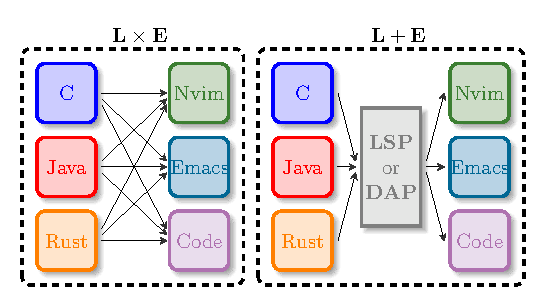
\includegraphics[width=0.75\linewidth]{figs/lsp_combinations.pdf}
    \caption{Traditional approach to language support in editors.}
    \label{fig:traditional}
\end{figure}
In this context, Microsoft in 2016 proposed the \textit{Language Server Protocol} and the \textit{Debugger Adapter Protocol} for Visual Studio Code as a promising solution to this problem, reducing from $\mathcal{L} \times \mathcal{E}$ to $\mathcal{L} + \mathcal{E}$ the number of combinations to be implemented, as it decouples the implementation of the language support from the editor (see Figure~\ref{fig:traditional}).
Detailing, the LSP and DAP are protocols that describes a common \textit{Application Programming Interface} (API) that the \textbf{language server} (LS) should implement, with the benefit of having only one implementation of the LS and multiple clients (IDEs and SCEs) that can consume it, essentially establishing a \textit{client-server} relationship through a communication channel (e.g., \textit{pipes} or \textit{sockets}).
owever, the implementation of an LS and its integration with an IDE/SCEs is still a complex task, as it requires the knowledge of the LSP specification and the implementation of the language support.
The implementation~\cite{Gunasinghe22} of an LS is done entirely manually and it is a \textit{top-down} activity, where most of the time is spent on the design and implementation data structures and algorithms.
Recently, researchers have started talking about the \textit{Software Product Lines} (SPLs) \cite{Cazzola23d, Cazzola20} to move towards a more modular world, where the implementation of a software system can be done in a compositional way, by composing the features of the SPL.
When a SPL is applied to the implementation of a programming language, each product corresponds to a language variant \cite{Cazzola15f} taking the name of \textit{Language Product Lines} (LPLs) \cite{Cazzola15f}. LPLs have been successfully used in both GPLs \cite{Cazzola16, Cazzola16i, Cazzola15f} and DSLs \cite{Haugen08, Liebig13, Cazzola14e, Wende09, White09}.
\hfill \break
\begin{figure}[t]
    \centering
    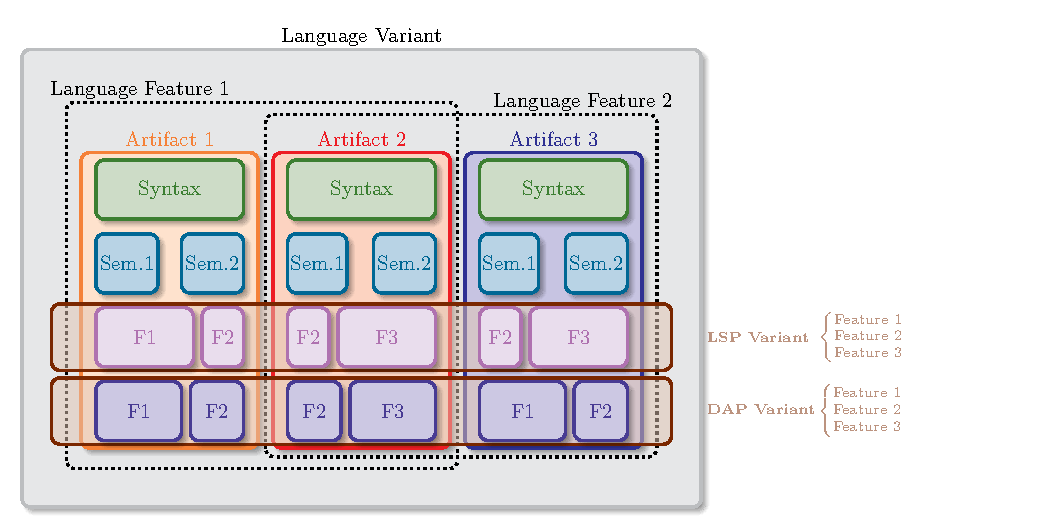
\includegraphics[width=0.9\linewidth]{figs/module_with_lsp.pdf}
    \caption{Proposed approach to modular implementation of LSP and DAP.}
    \label{fig:proposed}
\end{figure}
What I want to prove with this project is that the implementation of an LS could be a \textit{bottom-up} activity, where each LSP or DAP functionality can be see as a separate \textit{feature module} \cite{Batory04, Kastner11} splitted across the language artifacts, where each artifacts can be part of one or more \textit{features} (see Figure~\ref{fig:proposed}). These units can be composed to provide a modular implementation of the LS. This approach is supported by the fact that the LSP and DAP are \textit{language-agnostic} protocol \cite{Niephaus20, Rodriguez-Echeverria18}, which means that it does not impose any restrictions on the implementation of the LS, as long as it respects the specification of the protocol.
In \textit{feature-oriented programming} (FOP) \cite{Apel13, Czarnecki04, Prehofer01}, a feature module is a unit of composition that encapsulates a specific functionality, and it is a first-class entity that can be composed with other feature modules to form a software system; similar to an aspect module that encapsulates a crosscutting concern in \textit{aspect-oriented programming} (AOP) \cite{Kiczales01, Kiczales97, Laddad03}.
So, proponing a new modular approach to the implementation of an LS, based also on FOP, I want to extend Neverlang Language Workbench~\cite{Cazzola15c, Cazzola14c} in order to give support to the implementation of the LS for each semantic action of the language, and I will also implement the Neverlang LSP~\cite{Cazzola19} and DAP to support the composition of the LS feature modules.
In this way, the implementation of the LS is a \textit{bottom-up} activity, where each semantic action has attached a feature module that implements the LS functionality for that action, and these units can be composed to provide a modular implementation of the LS.
Each feature module will be written using a DSL, developed in the context of the Neverlang framework, that is specific for the implementation of the LS, and it is independent from the language for which the LS is being implemented.
Furthermore, with this approach, we want to prove that it is possible to reduce the number of combinations from $\mathcal{L} + \mathcal{E}$ to $\mathcal{L} \times 1$ by generating client implementations.

\hfill \break
\noindent
\textbf{Methodology}

The first step involves defining feature modules, which are essential components that encapsulate different functionalities of Language Server Protocol (LSP) and Debug Adapter Protocol (DAP). These functionalities include syntax highlighting, code completion, debugging, and documentation support. Each feature module is identified and defined based on its specific role within the LSP and DAP ecosystem. Following the identification of feature modules, the next phase is developing domain-specific languages (DSLs) within Neverlang. These DSLs are tailored to facilitate the development and composition of the feature modules, providing a structured and efficient way to create and manage them. Once the feature modules are defined and the DSLs are developed, the next step is to implement a system within Neverlang that allows for the composition of these feature modules. This system enables the integration of various feature modules into a complete and functional Language Server. With the modular framework in place, the next phase involves developing Language Servers for multiple programming languages. This step demonstrates the reuse and compositional capabilities of the feature modules. By leveraging the modular design, Language Servers for different languages can be developed more efficiently and with greater consistency. To ensure the effectiveness of these Language Servers, their performance and integration within different Integrated Development Environments (IDEs) and Source Code Editors (SCEs) will be evaluated. This evaluation will focus on how well the Language Servers perform in real-world development environments and how seamlessly they integrate with existing tools. The final phase of the methodology involves a comprehensive comparison and analysis. This includes evaluating the effort and complexity involved in the modular approach compared to traditional top-down methods. By analyzing the development process, the benefits and challenges of using a modular framework can be assessed. Additionally, the maintainability and extensibility of the modular approach will be scrutinized. This involves introducing changes and enhancements to the Language Servers and observing how easily these modifications can be implemented. The goal is to determine whether the modular approach offers superior maintainability and extensibility compared to traditional methods.

\hfill \break
\noindent
\textbf{Expected Contributions}

\begin{itemize}
    \item \textbf{A Modular Framework for Language Server Development}: A comprehensive framework within the Neverlang Language Workbench that supports the modular development of Language Servers.
    \item \textbf{Reduction in Development Effort}: Empirical evidence demonstrating a reduction in the development effort and complexity associated with implementng Language Servers.
    \item \textbf{Reusable and Language-Agnostic Modules}: A library of reusable, language-agnostic feature modules for common LSP and DAP functionalities.
    \item \textbf{Case Studies and Practical Applications}: Detailed case studies showcasing the practical applications of the modular approach across different programming languages and development environments.
\end{itemize}


\hfill \break
\noindent
\textbf{Timeline}

\hfill \break
\begin{figure}[t]
    \centering
    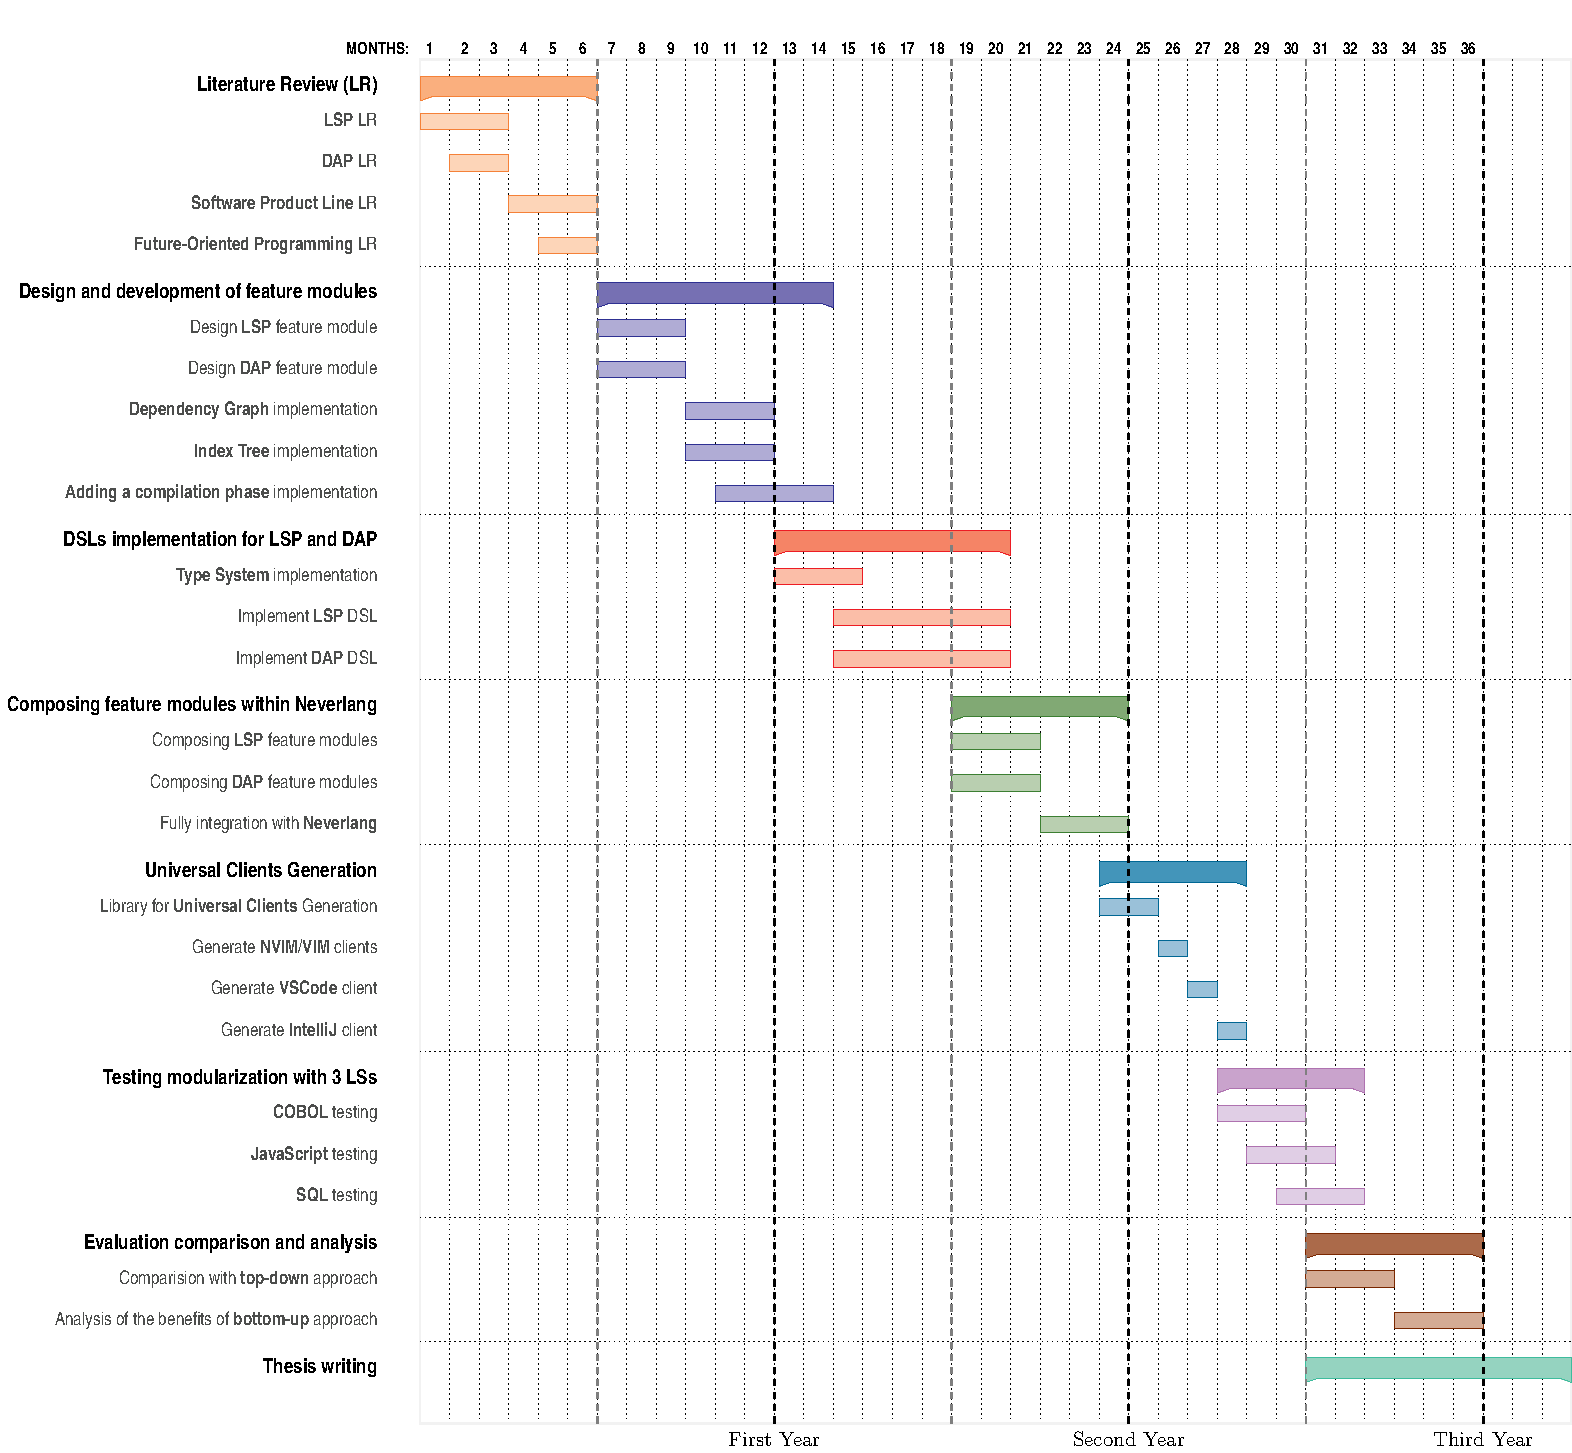
\includegraphics[width=.9\linewidth]{figs/gantt.pdf}
    \caption{Proposed timeline for the research project.}
    \label{fig:gantt}
\end{figure}

In figure \ref{fig:gantt} is shown the proposed timeline for the research project. The project is divided into seven main phases:
\begin{itemize}
    \item Literature Review
    \item Design and development of feature modules
    \item DSLs implementation<D-s>for LSP and DAP
    \item Composing feature modules within Neverlang
    \item Universal Clients Generation
    \item Testing modularization with 3 LSs
    \item Evaluation comparison and analysis
\end{itemize}

The literature phase will be carried out in the first six months. I will start by expanding my knowledge LSP and DAP in general, and then I will perform a deeper study of all the most important approaches currently available in literature to elaborate on their pros and cons and lay a groundwork for my research work. Great attention would be given to the study of bottom-up and top-down approaches, in order to find their shared aspects. This process will lead to the drafting of a survey on feature-oriented programmin and software product lines.
During the next eight months, I will design and develop the feature modules for the LS, and I will extend the Neverlang framework to support the implementation of the LS feature modules. This will be supported by the implementation of generic data structures, such as \textit{Indexed Trees}, \textit{Dependency Graphs}, and \textit{Symbol Tables}, that will be populated by any given language artifact not known \textit{a priori}. An additional compilation step will be added to the Neverlang framework to generate the feature modules from the language artifacts.
In the following eight months, I will implement the DLSs for the LSP and DAP, and I will extend the Neverlang framework to support the composition of the LS feature modules through the DLSs. This will be supported by the implementation of a \textit{multi-dimensional variability model}~\cite{Rosenmuller11}.
One of the biggest challenges, in the next six months, will be to compose the feature modules. This will be done by implementing a \textit{composition algorithm} that will take as input the splitted feature modules and the language artifacts and will produce the LS feature module.
The following six months will be dedicated to the generation of the universal clients. This will be done by implementing a \textit{client generator} that will take as input the LS feature module and will produce the client implementation. This will be supported by the implementation of a \textit{client language} that will allow the developer to specify which client to generate. The client generator will be able to generate clients for different IDEs and SCEs, such as Visual Studio Code, Vim/Nvim and IntelliJ IDEA.
In the last six months, I will test the modularization with three LSs, evaluating the feasibility of the approach. This will be done by implementing the LS for three different languages and by generating the client implementations. The evaluation will focus on the effort and complexity involved in the development of the LS, the maintainability and extensibility of the LS, and the integration of the LS with the existing tools. The evaluation will also include a comparison with the traditional approach to LS development, to assess the benefits and challenges of using the modular framework.




\hfill \break
\noindent
\textbf{Conclusion}

The proposed modular approach to implementing Language Servers via feature-oriented programming within the Neverlang Language Workbench represents a significant advancement in reducing the complexity and effort associated with developing Language Servers. By decomposing the LS functionalities into reusable and composable feature modules, this approach promises to enhance maintainability, extensibility, and overall efficiency in the development of language support tools. This research will contribute valuable insights and practical solutions to the field of programming language implementation and development environment integration.
Considering the potential impact of this research, I am confident that the proposed project will yield valuable contributions to the field of programming language development and integration. By providing a modular framework for the implementation of Language Servers, this research has the potential to revolutionize the way language support tools are developed and maintained. The reduction in development effort, the increased reusability of feature modules, and the improved maintainability and extensibility of Language Servers are just a few of the benefits that this research aims to deliver. With the proposed timeline and methodology, I am confident that this research project will be completed successfully and will make a significant contribution to the field of programming languages.
